%% IOP - architektura systemu
%

\documentclass[a4paper]{article}

\usepackage[utf8]{inputenc}
\usepackage{polski}
\usepackage{fullpage}
\usepackage{graphicx}

\title{Opis architektury do projektu ,,System rozproszonej kompilacji''}
\author{Marta Drozdek, Anna Lewicka, Wacław Banasik, Mateusz Machalica}
\date{\today}

\begin{document}

\maketitle

\begin{table}[!h]
	\centering
	\begin{tabular}{|c|c|c|p{8cm}|}
		\hline
		\textbf{Data} & \textbf{Wersja} & \textbf{Autorzy} & \textbf{Opis zmian} \\ \hline
		19/03/2012 & 1 & Marta Drozdek & Dokumentacja pierwszego projektu architektury \\ \hline
		30/05/2012 & 2 & Mateusz Machalica & Nowy opis architektury systemu, diagramy podziału na podsystemy i moduły oraz schemat przepływu sterowania \\ \hline
	\end{tabular}
\end{table}

\section{Wstęp}

Celem tego dokumentu jest opis architektury systemu i decyzji projektowych podjętych celem spełnienia wymagań pozafunkcjonalnych.
Wymagania dotyczące systemu zostały sformułowane w osobnym dokumencie -- ,,Wymaganiach projektu''.

\input{slownik_pojec.tex.inc}

\section{Ogólne założenia odnośnie architektury systemu}

Architektura systemu powinna zapewniać łatwość w rozszerzaniu możliwości działania systemu przy użyciu równych mechanizmów zdalnego wykonywania poleceń i synchronizacji plików.
Dlatego też te podsystemy powinny składać się z modułów implementujących wspólny interfejs, niezależny od technologii komunikacyjnej użytej do implementacji funkcjonalności danego modułu.

\section{Podział na podsystemy}

Poniżej prezentujemy diagram podziału systemu na podsystemy i moduły, po nim następuje opis każdego podsystemu i zawartych w nim modułów.

\begin{figure}[h!t]
	\centering
	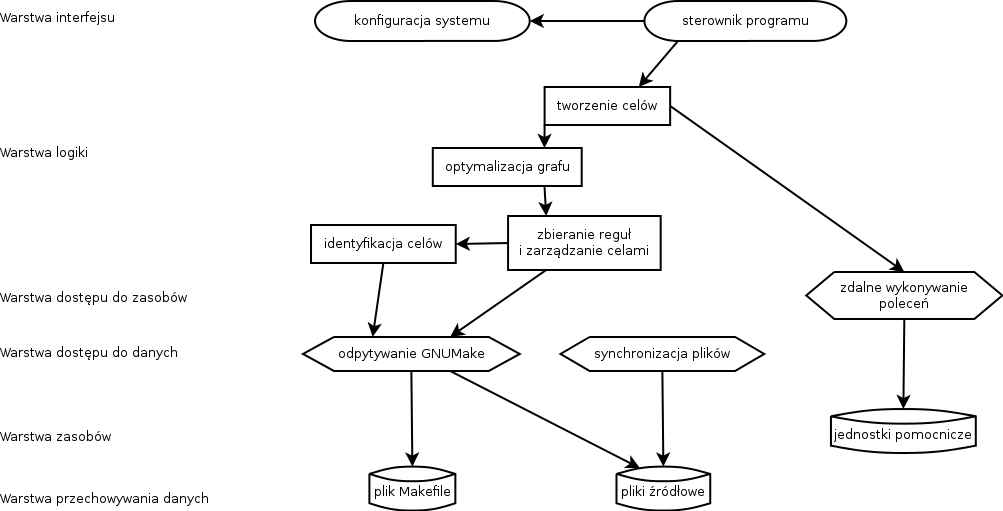
\includegraphics[width=450px]{architektura_podsystemy.png}
	\caption{Schemat architektury systemu wraz z zależnościami pomiędzy modułami i podsystemami. Wyróżniono dwie dodatkowe warstwy -- zasoby, które nie są danymi wejściowymi i moduły dostępu do nich \label{fig:arch}}
\end{figure}

\subsection{Moduł interpretatora poleceń i sterownika}

Zadaniem tego modułu jest podjęcie decyzji o rozpoczęciu kompilacji z odpowiednimi parametrami po przetworzeniu opcji przekazywanych w linii komend.
Moduł ten wywołuje inne podsystemy w odpowiedniej kolejności po czym przekazuje sterowanie do podsystemu tworzenia celów i przejmuje z powrotem tuż przed zakończeniem programu.

\subsection{Moduł konfiguracji}

Zadaniem tego modułu jest odczytywanie konfiguracji i udostępnianie innym modułom i podsystemom.
Z racji oddelegowania konfiguracji związanej z procesem łączenia i autoryzacją jednostek pomocniczych do pliku konfiguracyjnego klienta SSH, konfiguracja systemu sprowadza się do podania nazw hostów pełniących funkcje jednostek pomocniczych i dodatkowych informacji jak katalog tymczasowy, w którym można wykonywać zdalnie przepisy.

W przyszłości dopuszczamy możliwość podawania w konfiguracji statycznych informacji o wydajności jednostek pomocniczych, na podstawie których podsystem koordynujący będzie decydował o rozdzielaniu zadań.

\subsection{Moduł odpytywania programu GNUMake}

Ze względów częstego odpytywania (wywoływania z odpowiednimi opcjami i parsowania wyników) programu GNUMake w podsystemie identyfikowania celów oraz podsystemie zbierania reguł i zarządzania aktualnymi celami, pomocnym okazało się stworzenie osobnego modułu, którego jedynym zadanie będzie usystematyzowanie komunikacji z programem GNUMake w formie wygodnego interfejsu.

Ilekroć dalej piszemy, że podsystem lub moduł uzyskuje informacje od programu GNUMake, to w domyśle dopowiadamy, że dokonuje tego poprzez użycie tego modułu.

\subsection{Podsystem identyfikowania celów i budowy grafu zależności}

Zadaniem tego podsystemu jest wyekstrachowanie z pliku Makefile struktury grafu zależności, to znaczy nazw celów i zależności pomiędzy nimi i zbudowanie grafu, w którym wierzchołkami są cele, a krawędź skierowana (A, B) należy do grafu wtedy i tylko wtedy, gdy B zależy od A.
W praktyce w grafie będziemy trzymać zarówno krawędzie jak zdefiniowano powyżej jak i krawędzie odwrócone, jako osobne zbiory krawędzi.

Celem zachowania zgodności z ,,implicit targets'' zdefiniowanymi w standardzie GNUMake, system wykorzystuje do identyfikacji celów i zależności sam program GNUMake, który umożliwia wykonanie na standardowe wyjście zrzutu bazy danych tworzonej na podstawie pliku Makefile, która zawiera pełną informację potrzebną do zbudowania celów opisanych pliku Makefile.
Parsując zrzut bazy danych jesteśmy w stanie odtworzyć strukturę grafu zależności.

Po zbudowaniu grafu podsystem sprawdza, czy nie ma w nim cyklu zależności i jeśli jest, to zgłasza błąd informując, że takowy cykl wykrył.

\subsection{Podsystem zbierania reguł dla celów i zarządzania aktualnymi celami}

Celem tego podsystemu jest uzupełnienie grafu zależności zbudowanego przez podsystem identyfikowania celów o przepisy (ciągi instrukcji i podprogramów, które należy wykonać aby zbudować dany cel) dla każdego celu.
Ponadto podsystem przy uzupełnianiu grafu kompilacji bierze pod uwagę już zbudowane cele, które nie muszą zostać ponownie skompilowane. Do oceny, czy dany cel wymaga ponownego przebudowania, a więc czy ciąg instrukcji koniecznych do jego wykonania nie jest pusty, wykorzystywane są daty modyfikacji plików zapewniane przez lokalny system plików.

W przypadku, gdy takie informacje są niedostępne, kompilacja przebiega tak, jakby wszystkie pliki źródłowe zostały zaktualizowane i wszystkie cele (również pośrednie) musiały zostać ponownie skompilowane.
Potencjalnie możliwe jest w takiej sytuacji ponowne skompilowanie wszystkich celów, pomimo ich aktualności.
Trudno jednak wyobrazić sobie, aby taka sytuacja -- działanie na danych trzymanych w systemie plików bez wsparcia dla czasów modyfikacji -- miała miejsce często.
Ponadto powyższe zachowanie jest zgodne z zachowaniem programu GNUMake w opisanej sytuacji.

Aby zapewnić jak największą zgodność z pierwowzorem i implementować wszystkie specyficzne możliwości programu GNUMake, jak ekspansja zmiennych i zmienne domyślne w plikach Makefile, do uzupełniania grafu zależności stosujemy informacje uzyskane od programu GNUMake wywołanego dla danego pliku Makefile.

\subsection{Moduł optymalizacji grafu kompilacji}

Zadaniem tego modułu będzie optymalizacja gotowego grafu kompilacji.
Danymi wejściowymi będzie graf kompilacji utworzony przez podsystem identyfikacji celów i uzupełniony o reguły przez podsystem zbierania reguł.
Efektem ma być zmodyfikowany graf opisujący równoważny proces kompilacji, to znaczy prowadzący do takich samych plików wynikowych.
Dopuszczamy dowolne modyfikacje struktury grafu, jeśli nie narusza one poprawności, to znaczy ostateczny efekt wykonania kompilacji według nowego grafu ma być taki sam jak według grafu sprzed modyfikacji.

Przykładowym sposobem optymalizacji może być skracanie ścieżek złożonych z celów, których kompilacje nie może być zrównoleglona.
Poprzez potraktowanie ich jako jednego celu zyskujemy na szybkości kompilacje poprzez ograniczenie narzutów sieciowych i na dystrybucję zadań oraz synchronizację plików źródłowych.

W początkowych wydaniach moduł ten będzie nieobecny -- doążymy do tego, aby najpierw cały system działał poprawnie, dopiero potem zajmiemy się jego optymalizacją.

\subsection{Podsystem tworzenia celów i koordynowania procesu kompilacji}

Zadaniem procesu tworzenia celów jest skoordynowanie działania innych podsystemów, tak aby w efekcie otrzymać skompilowane żądane cele, opisane w grafie zależności, \emph{w jak najkrótszym czasie}.

Aby to osiągnąć wykonujemy równolegle maksymalną liczbę przepisów, musimy jednak respektować zależności łączące cele.
Ponieważ w grafie zależności nie ma cykli (podsystem identyfikacji celów zgłosiłby wtedy błąd), możemy w trakcie sortowania topologicznego grafu wykonywać równolegle wszystkie przepisy, na których zrównoleglenie pozwala nam struktura grafu.

\subsection{Podsystem zdalnego wykonywania poleceń}

Każdy protokół zdalnego wykonywania poleceń, jaki uznajemy za odpowiedni do użycia w projekcie, działa w architekturze klient-serwer, gdzie klientem jest komputer zlecający wykonanie polecenia, w naszym przypadku jednostka koordynująca, natomiast rolę serwera pełni jednostka pomocnicza.

Chcemy przenieść ten modela na interakcję podsystemu tworzenia celów i podsystemu zdalnego wykonywania poleceń.
Do dyspozycji podsystemu koordynującego proces kompilacji będzie pozostawała pewna pula obiektów reprezentujących lokalne procesy, które są połączone przy pomocy dostępnych środków komunikacyjnych (SSH lub RSH) z jednostkami pomocniczymi.
Każdy obiekt z tej puli udostępnia, niezależnie od wykorzystywanego środka komunikacji, taki sam interfejs do zlecania wykonania pewnych zadań, odbierania wyników tych zadań (ewentualnie informowania o błędach), a także wymuszania zakończenia realizacji danego zadania.

Zadania zlecone takiemu obiektowi są realizowane na jednostce pomocniczej i po zakończeniu wykonania, wyniki są przesyłane do jednostki koordynującej.
Obiekt informuje o powodzeniu lub błędzie (podając przyczynę) wykonania zadania i zgłasza gotowość do ponownego użycia.

Chcemy jeszcze raz podkreślić, że interfejs udostępniany przez różne moduły realizujące zdalne wykonywanie poleceń ma być identyczny, podsystem koordynowania procesu kompilacji nie musi zatem rozróżniać obiektów pochodzących z różnych modułów.

Celem redukcji nakładu pracy i ryzyka popełnienia błędów rzutujących na bezpieczeństwo systemu, do implementacji poniższych modułów modułu zaleca się wykorzystanie istniejących bibliotek.

\subsubsection{Moduł obsługi SSH}

Jednym z modułów zapewniających zdalne wykonywanie poleceń jest moduł wykorzystujący do komunikacji protokół SSHv2.
Moduł ten powinien być stosowany do komunikacji w sieciach rozległych lub gdy komunikacja nie powinna być podsłuchiwana, a nie mamy zaufania do wykorzystywanej infrastruktury sieciowej.
Coraz częściej SSH jest jedynym dostępnym rozwiązaniem 

\subsubsection{Moduł obsługi RSH}

Docelowo zamierzamy dostarczać możliwość wykorzystania RSH do komunikacji w zaufanej sieci lokalnej.
Coraz częściej jednak oprogramowanie to nie jest instalowane z racji niskiego poziomu bezpieczeństwa, stąd moduł ten zostanie zaimplementowany w dalszych iteracjach projektu.

\subsection{Podsystem synchronizacji plików}

Podobnie jak w podsystemie zdalnego wykonywania poleceń, również tutaj zamierzamy udostępniać rożne moduły implementujące odmienne metody i protokoły wymiany plików źródłowych oraz pośrednich, których interfejsy będą zgodne.

Poza informacjami zawartymi w grafie kompilacji, drugim źródłem danych wejściowych są pliki znajdujące się w katalogu, w którym ma przebiegać kompilacja.
Celem opisywanego podsystemu jest dostarczenie mechanizmów od wymiany plików pomiędzy jednostkami pomocniczymi i jednostką koordynującą na zasadzie oddania w użytkowanie danych z koniecznością zwrotu wraz z wynikami obliczeń do jednostki koordynującej.

Taki scentralizowany schemat serwowania plików źródłowych ma zarówno wady jak i zalety.

Jako wadę można wymienić duże obciążenie łącza i procesora maszyny koordynującej.
Ponieważ jednak w domyśle na jednostce koordynującej nie są wykonywane inne obliczenia niż przetwarzanie grafu i zlecanie zadań jednostkom wykonującym, obciążenia procesora jest dopuszczalnym skutkiem ubocznym takiego schematu, jednak problem wysycania łącza tej maszyny pozostaje.

Istotnymi zaletami są natomiast: łatwość zarządzania zaktualizowanymi celami przy obliczaniu poleceń koniecznych do przebudowania kodu oraz zachowanie zgodności pod względem efektu końcowego użycia naszego systemu z pierwowzorem -- programem GNUMake.

Częściowym rozwiązaniem problemu obciążenia łącza jednostki koordynującej można próbować rozwiązać stosując rozproszony system plików, którego węzłami przechowującymi dane byłyby również jednostki pomocnicze, jednak wtedy tracimy łatwość konfiguracji i uruchamiania systemu oraz dalej nie mamy gwarancji, że ruch w sieci ulegnie zmniejszeniu.
Nie mając kontroli nad algorytmami klastrującymi i rozdzielającymi dane na poszczególne węzły, może się okazać, że każdej jednostce pomocniczej przypiszemy zadania wymagające dostępu do plików, które znajdują się na innej maszynie.

Poniżej opisano dwa moduły, których implementacja i testowanie powinno być rozważone w pierwszym rzędzie.

\subsubsection{Moduł NFS}

W przypadku pracy w sieci lokalnej naturalnym pomysłem wydaje się zastosowanie do wymiany plików sieciowego systemu plików NFS.
Można wtedy nie implementować żadnych dodatkowych mechanizmów synchronizacji, gdyż instancja NFS ze wspólnym zasobem podmontowanym na każdej jednostce pomocniczej i jednostce koordynującej gwarantuje, że wszystkie te komputery pracują na tym samym drzewie katalogów i zawartości plików.

Taki schemat wymiany plików powoduje, że obciążenie jednostki koordynującej jest znikome, natomiast komputer pełniący funkcję serwera przejmuje całe obciążenie związane z synchronizacją plików.
Naturalnie może się okazać, że serwer plików i jednostka koordynująca to ta sama maszyna.

Z racji prostoty i akceptowalnej wydajności takiego rozwiązania powinien być to pierwszy wybór, jeśli mamy do dyspozycji szybką sieć i pulę komputerów z dostępem do wspólnego zasobu NFS.

\subsubsection{Moduł SSHFS}

Jako system plików w przestrzeni użytkownika SSHFS zapewnia niższa wydajność niż rozwiązania pracujące w przestrzeni jądra, jak na przykład sterowniki systemu plików NFS.
Niezaprzeczalną zaletą wymiany plików przy pomocy SSHFS jest jej bezpieczeństwo, gdyż jako protokołu transportowego system ten używa SSH.
W sieciach niezaufanych jest rozwiązanie dużo lepsze niż próba dostosowania systemu NFS do operowania w takich warunkach.
Ponadto konfiguracja instancji NFS jest bardzo skomplikowana w porównaniu z konfiguracją oprogramowania SSHFS.

Wykorzystanie systemu SSHFS niesie już opisane wady.
Ponieważ serwerem plików jest w takiej konfiguracji jednostka koordynująca, to łącze tej maszyny będzie silnie obciążone.
Ponadto wykorzystanie procesora wzrośnie wielokrotnie z racji szyfrowania danych.
Nadzieję w tej kwestii niesie coraz częstsze wbudowywanie specjalnych instrukcji przyspieszających szyfrowanie przez producentów procesorów w swoje produkty przeznaczone na rynek użytkowników domowych. Dla przykładu prędkość szyfrowania danych przy pomocy algorytmu AES z 256-bitowym kluczem na laptopie z 2010 roku (średnia klasa cenowa) wynosi około 120 MB/s.

Stąd możliwość zastosowania systemu SSHFS powinna być wykorzystywana tylko wtedy, gdy przedkładamy bezpieczeństwo transmisji nad jej prędkość.

\section{Przepływ sterowania}

%TODO diagram przepływu sterowania

Proces tworzenia i przekształcania grafu do ostatecznej postaci jest zrealizowany na zasadzie modelu potoków i filtrów -- kolejne podsystemy łączą dane wejściowe .
Wyjściem każdego etapu jest wzbogacona wersja grafu zależności stanowiąca jednocześnie jedno z wejść dla kolejnego etapu.
Kolejne podsystemy działają na grafie sekwencyjnie, jednak nie ma to zauważalnego wpływu na wydajność programu, natomiast znakomicie ułatwia implementację.

Z kolei w podsystemie koordynacji zadań przepływ sterowania rozdziela się na wiele procesów, przy czym podsystem koordynacji działa w trybie klienta, wysyłając do serwera -- podsystemu zdalnego wykonywania poleceń żądania (być może wiele na raz) i oczekując odpowiedzi.

\section{Komunikacja pomiędzy podsystemami}

Współdzielenie danych pomiędzy podsystemami realizujemy na zasadzie wspólnego repozytorium danych, jakim będzie graf kompilacji.
Taki model zapewni wymaganą efektywność, gdyż dane o poszczególnych celach będą potrzebne w różnych przestrzeniach adresowych podprocesów realizujących budowę poszczególnych celów, w trudnych do przewidzenia momentach, uwarunkowanych działaniem sieci i jednostek pomocniczych, które z naszego punktu widzenia są zmiennymi losowymi.

Ponadto graf stanowi stosunkowo dużą porcję informacji i przekazywania go w komunikatach pomiędzy podsystemami stanowiłoby duży narzut czasowy.

Kolejnym argumentem przemawiającym za przyjęciem modelu repozytorium do współdzielenia danych jest jego naturalność dla tego systemu.
Każdy kolejny podsystem korzysta z informacji zawartych w grafie (potencjalnie wprowadzając niewielkie modyfikacje).
Sam obiekt grafu kompilacji jest kluczowym wyjściem dla jednych podsystemów i wejściem dla innych, można powiedzieć że działanie systemu ogranicza się tego przetwarzania grafu, stąd naturalnym wydaje się patrzenie na niego jak na główne repozytorium danych.

Zlecanie zadań innym podsystemom odbywać się ma na zasadzie przesyłania komunikatów, a dokładniej wywoływania metod odpowiednich obiektów reprezentujących podsystemy.

Poza informacjami zawartymi w grafie kompilacji, drugim źródłem danych wejściowych są pliki znajdujące się w katalogu, w którym ma przebiegać kompilacja.
Będą one zarządzane przez podsystem synchronizacji plików.
Model udostępniania tych danych, niezależnie od różnic dzielących moduły implementujące tą funkcjonalność, będzie przystawał do modelu repozytorium.
Głównym źródłem danych i miejscem, do którego są przesyłane po przetworzeniu wraz z wynikami jest katalog, w którym uruchomiono system na maszynie pełniącej funkcję jednostki koordynującej.

\end{document}
